\begin{activity} \label{8.3.Act4} Consider the harmonic series $ \sum_{k=1}^{\infty} \frac{1}{k}$. Recall that the harmonic series will converge provided that its sequence of partial sums converges. The $n$th partial sum $S_n$ of the series $ \sum_{k=1}^{\infty} \frac{1}{k}$ is
 \begin{eqnarray*}
 S_n & = & \sum_{k=1}^{n} \frac{1}{k} \\
 	& = & 1 + \frac{1}{2} + \frac{1}{3} + \cdots + \frac{1}{n} \\
 	& = & 1(1) + (1)\left(\frac{1}{2}\right) + (1)\left(\frac{1}{3}\right) + \cdots + (1)\left(\frac{1}{n}\right).
\end{eqnarray*}
Through this last expression for $S_n$, we can visualize this partial sum as a sum of areas of rectangles with heights $\frac{1}{m}$ and bases of length 1, as shown in Figure \ref{F:8.3.4_Integral_Test}, which uses the 9th partial sum.
\begin{figure}[h]
\begin{center}
\resizebox{!}{2.25in}{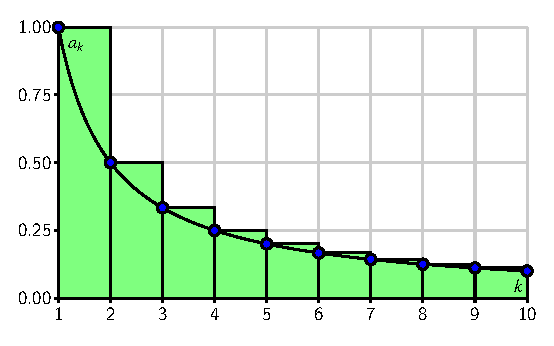
\includegraphics{figures/8_3_Integral_test1.eps}}
%\hspace{0.2in} \resizebox{!}{1.25in}{\includegraphics{figures/8.3_Integral_test2.eps}}
\caption{A picture of the 9th partial sum of the harmonic series as a sum of areas of rectangles.}
\label{F:8.3.4_Integral_Test}
\end{center}
\end{figure}
The graph of the continuous function $f$ defined by $f(x) = \frac{1}{x}$ is overlaid on this plot. 
\ba
\item Explain how this picture represents a particular Riemann sum.
\item What is the definite integral that corresponds to the Riemann sum you considered in (a)?
\item Which is larger, the definite integral in (b), or the corresponding partial sum $S_9$ of the series? Why?

\item If instead of considering the 9th partial sum, we consider the $n$th partial sum, and we let $n$ go to infinity, we can then compare the series $ \sum_{k=1}^{\infty} \frac{1}{k}$ to the improper integral $ \int_{1}^{\infty} \frac{1}{x} \ dx$.  Which of these quantities is larger?  Why?

\item Does the improper integral $ \int_{1}^{\infty} \frac{1}{x} \ dx$ converge or diverge? What does that result, together with your work in (d), tell us about the series $ \sum_{k=1}^{\infty} \frac{1}{k}$?

\ea
\end{activity}

\begin{smallhint}
\ba
	\item Small hints for each of the prompts above.
\ea
\end{smallhint}
\begin{bighint}
\ba
	\item Big hints for each of the prompts above.
\ea
\end{bighint}
\begin{activitySolution}
\ba
	\item Notice that the $n$th partial sum of the series $\ds \sum_{k=1}^{\infty} \frac{1}{k}$ is equal to the left hand Riemann sum of $f(x)$ on the interval $[1,n]$.
    \item Since $f$ is a decreasing function, it follows that
\[\ds \sum_{k=1}^{n} \frac{1}{k} > \int_{1}^{n} \frac{1}{x} \ dx.\]
    \item Letting Since $f$ is decreasing, the improper integral $\ds \int_{1}^{\infty} \frac{1}{x} \ dx$ is smaller than the limit of the Riemann sums as $n$ goes to infinity. So  we wind up with a comparison between the series $\ds \sum_{k=1}^{\infty} \frac{1}{n}$ and the improper integral:
\[\ds \sum_{k=1}^{\infty} \frac{1}{k} > \int_{1}^{\infty} \frac{1}{x} \ dx.\]
    \item We can evaluate the improper integral as follows:
\begin{align*}
\int_{1}^{\infty} f(x) \ dx &= \lim_{t \to \infty} \int_{1}^{t} \frac{1}{x} \ dx \\
    &= \lim_{t \to \infty} \ln(x) |_{1}^{t} \\
    &= \lim_{t \to \infty} \left(\ln(t) - \ln(1) \right) \\
    &= \infty.
\end{align*}
Since the value of the series $\ds \sum_{k=1}^{\infty} \frac{1}{k}$ exceeds the value of the infinite improper integral, we must conclude that the series $\ds \sum_{k=1}^{\infty} \frac{1}{k}$ diverges.
\ea
\end{activitySolution}
\aftera 